\begin{figure}
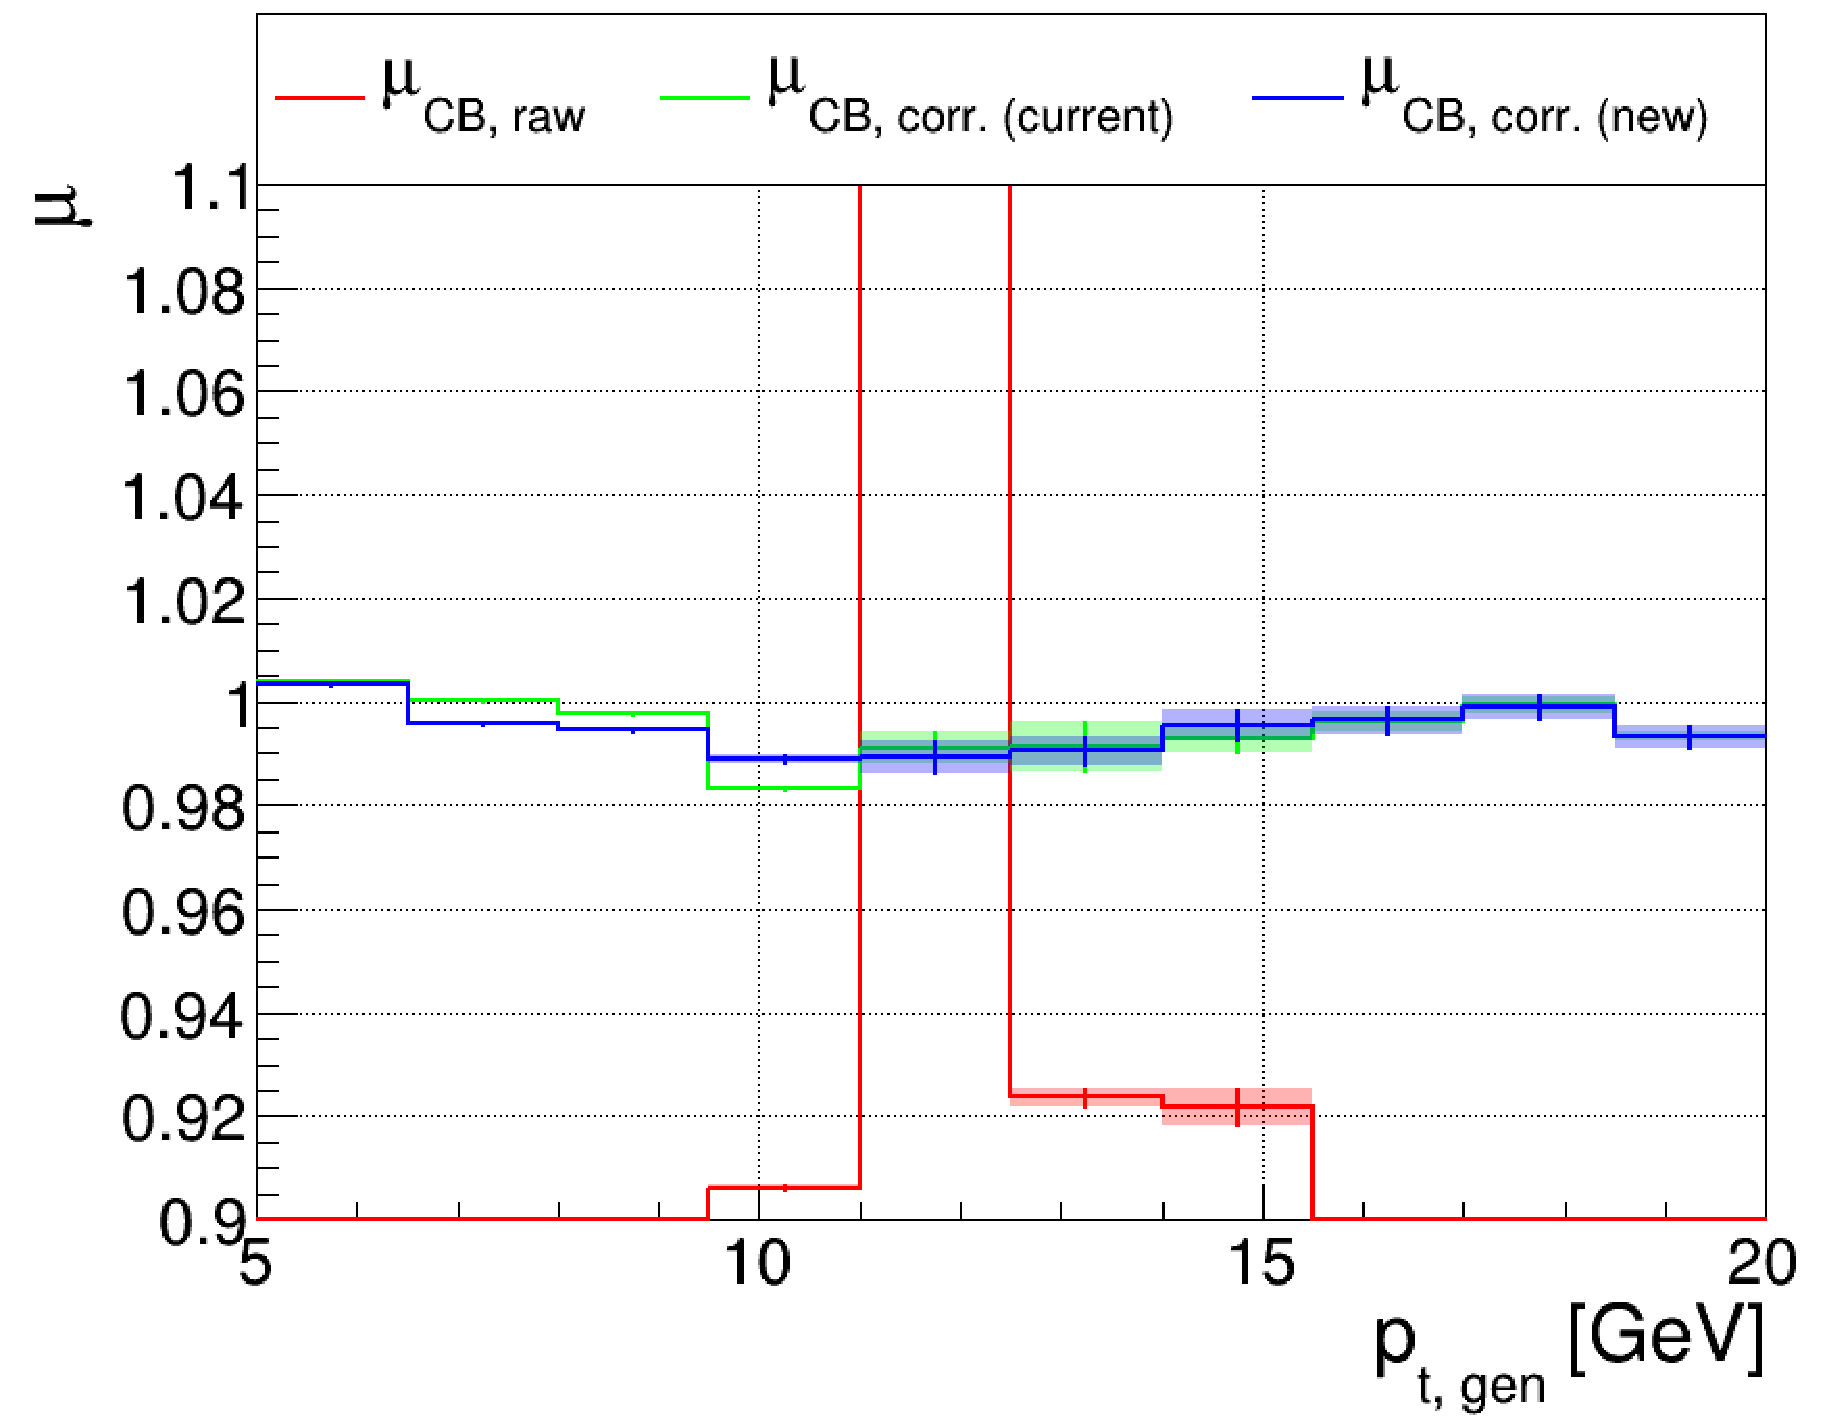
\includegraphics[width=0.495\textwidth]{./plots_pdf/ECAL_plots/plotsNoPU/EE/pdf/FULL/GENPT/EEFULL_GENPT_0005_0020_MuOverBins.pdf}
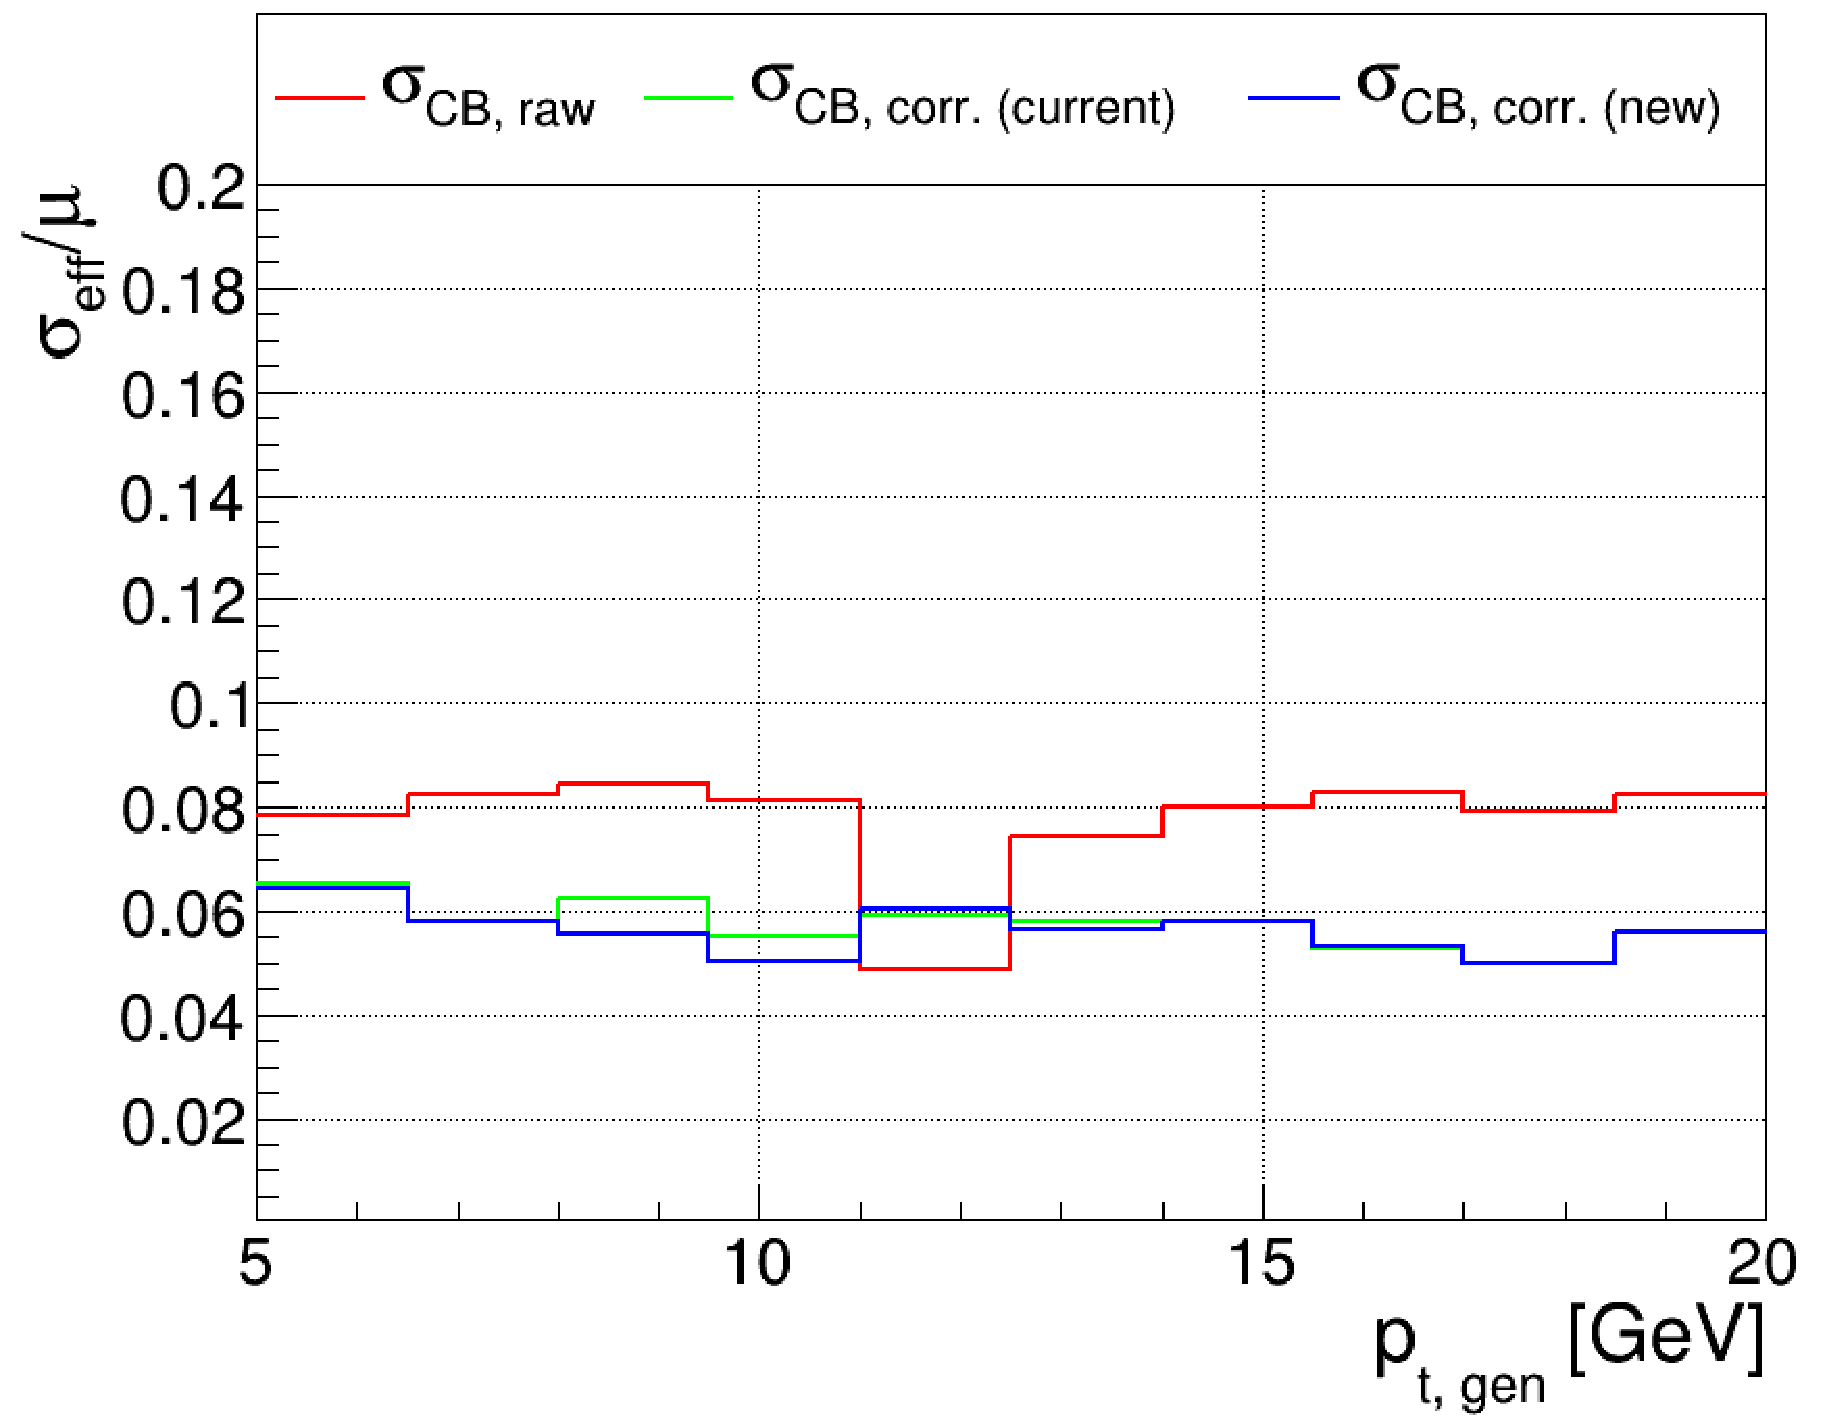
\includegraphics[width=0.495\textwidth]{./plots_pdf/ECAL_plots/plotsNoPU/EE/pdf/FULL/GENPT/EEFULL_GENPT_0005_0020_EffSigmaOverBins.pdf}
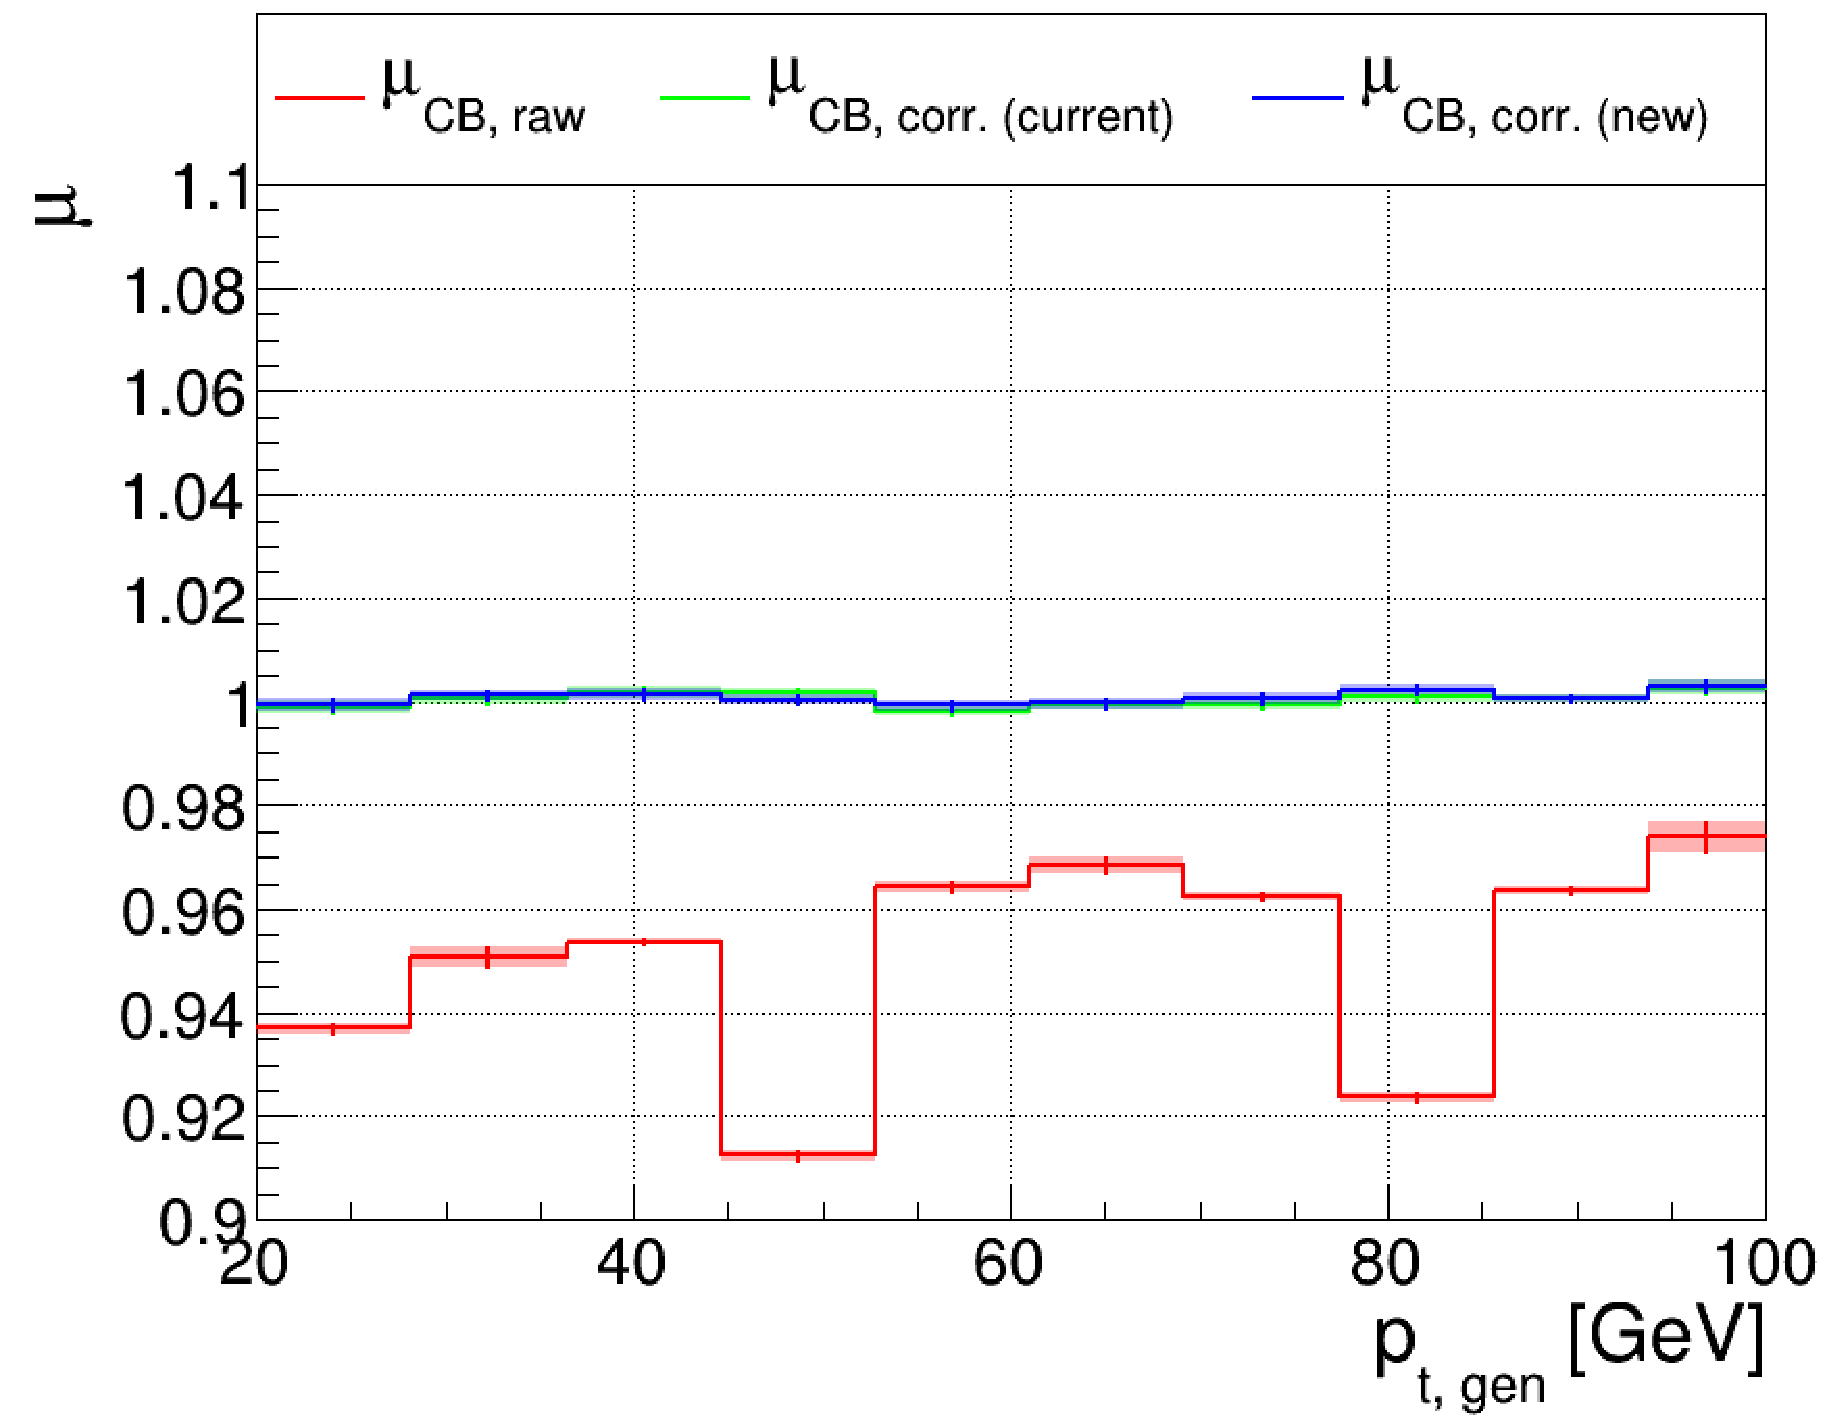
\includegraphics[width=0.495\textwidth]{./plots_pdf/ECAL_plots/plotsNoPU/EE/pdf/FULL/GENPT/EEFULL_GENPT_0020_0100_MuOverBins.pdf}
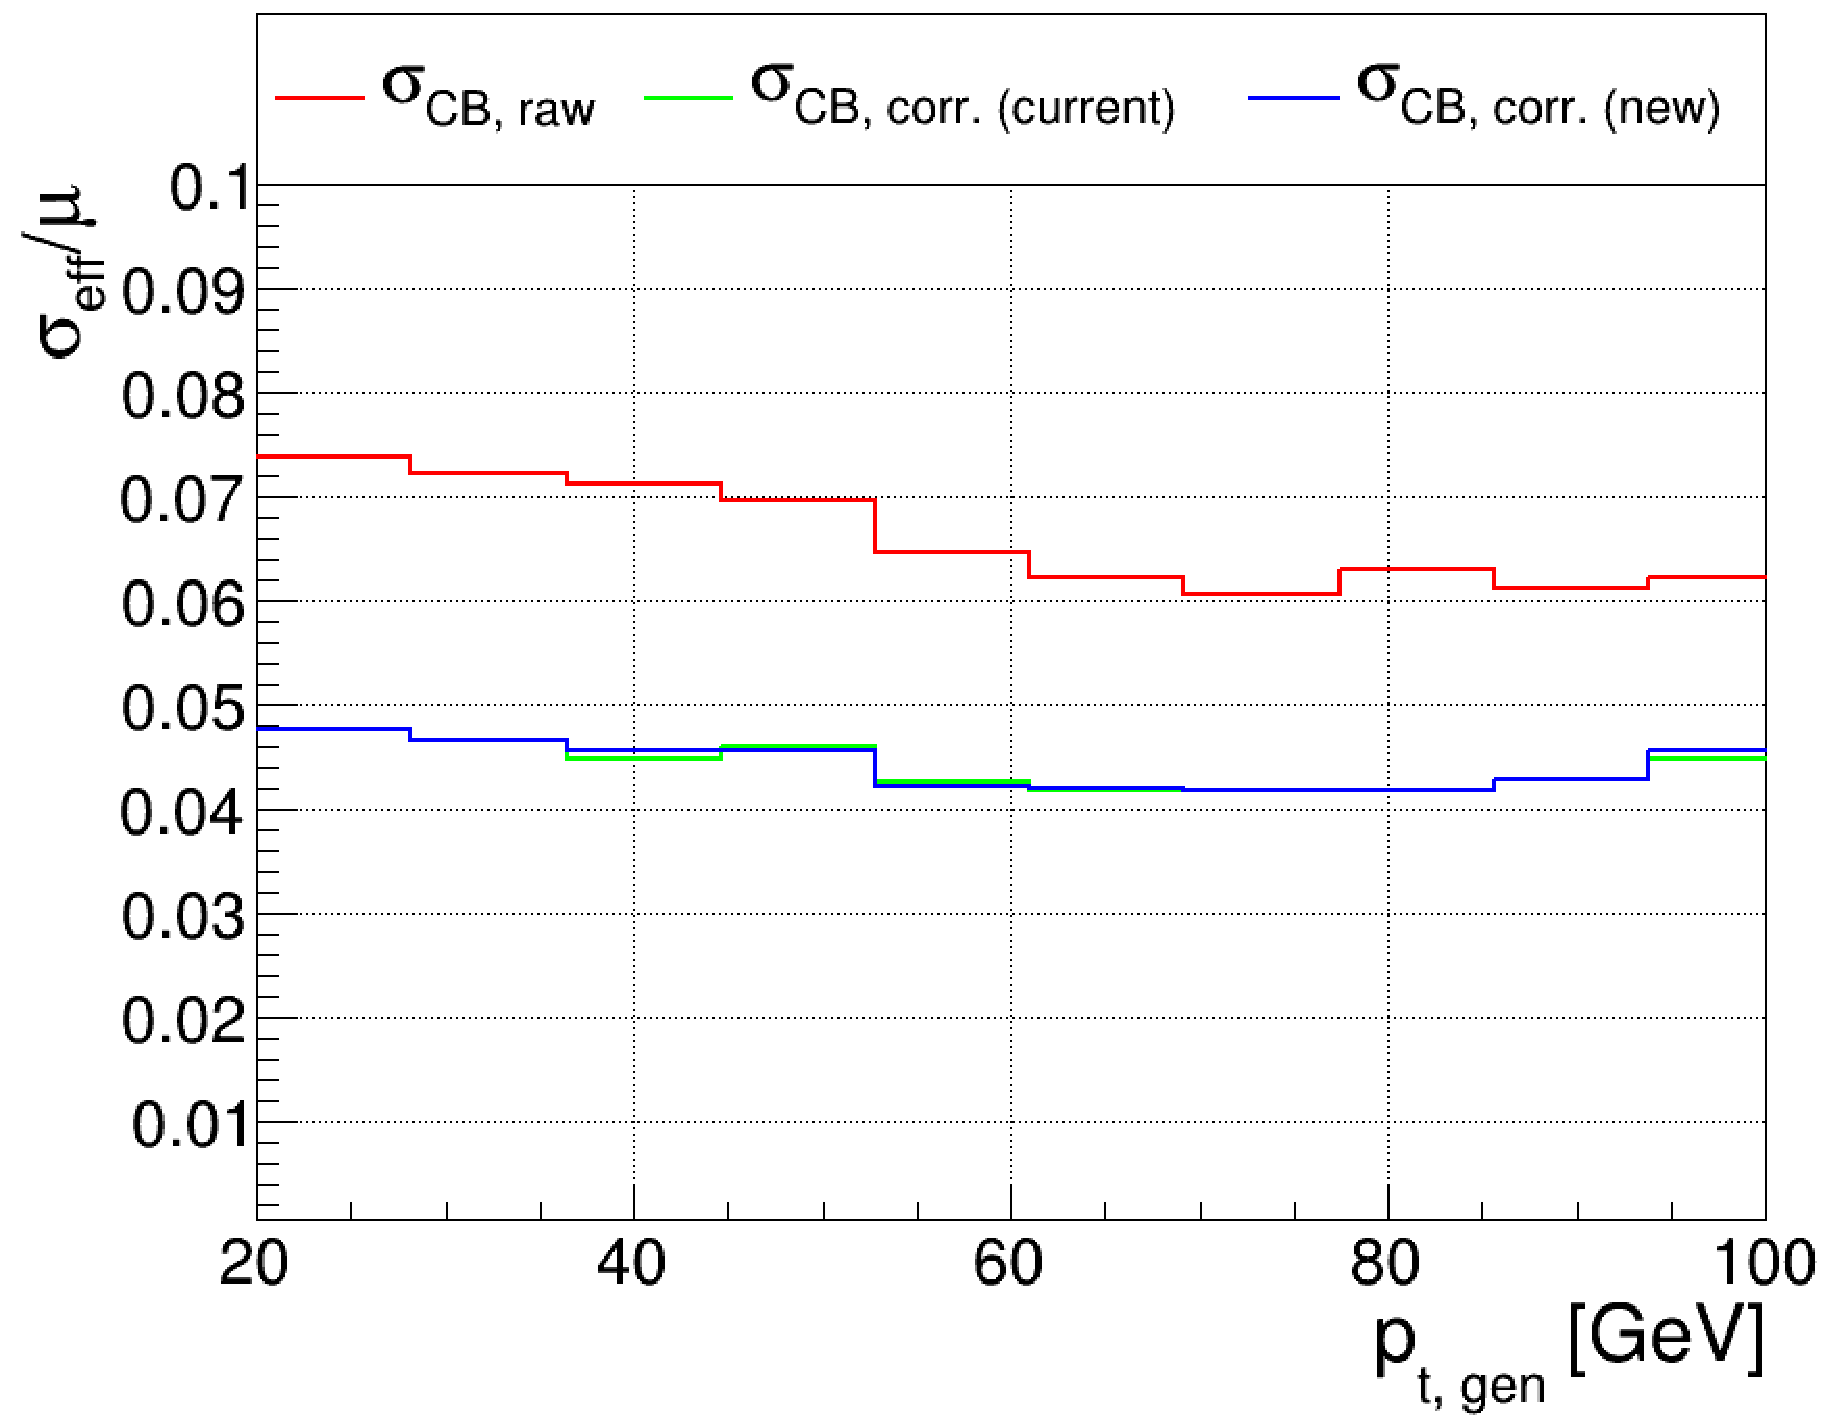
\includegraphics[width=0.495\textwidth]{./plots_pdf/ECAL_plots/plotsNoPU/EE/pdf/FULL/GENPT/EEFULL_GENPT_0020_0100_EffSigmaOverBins.pdf}
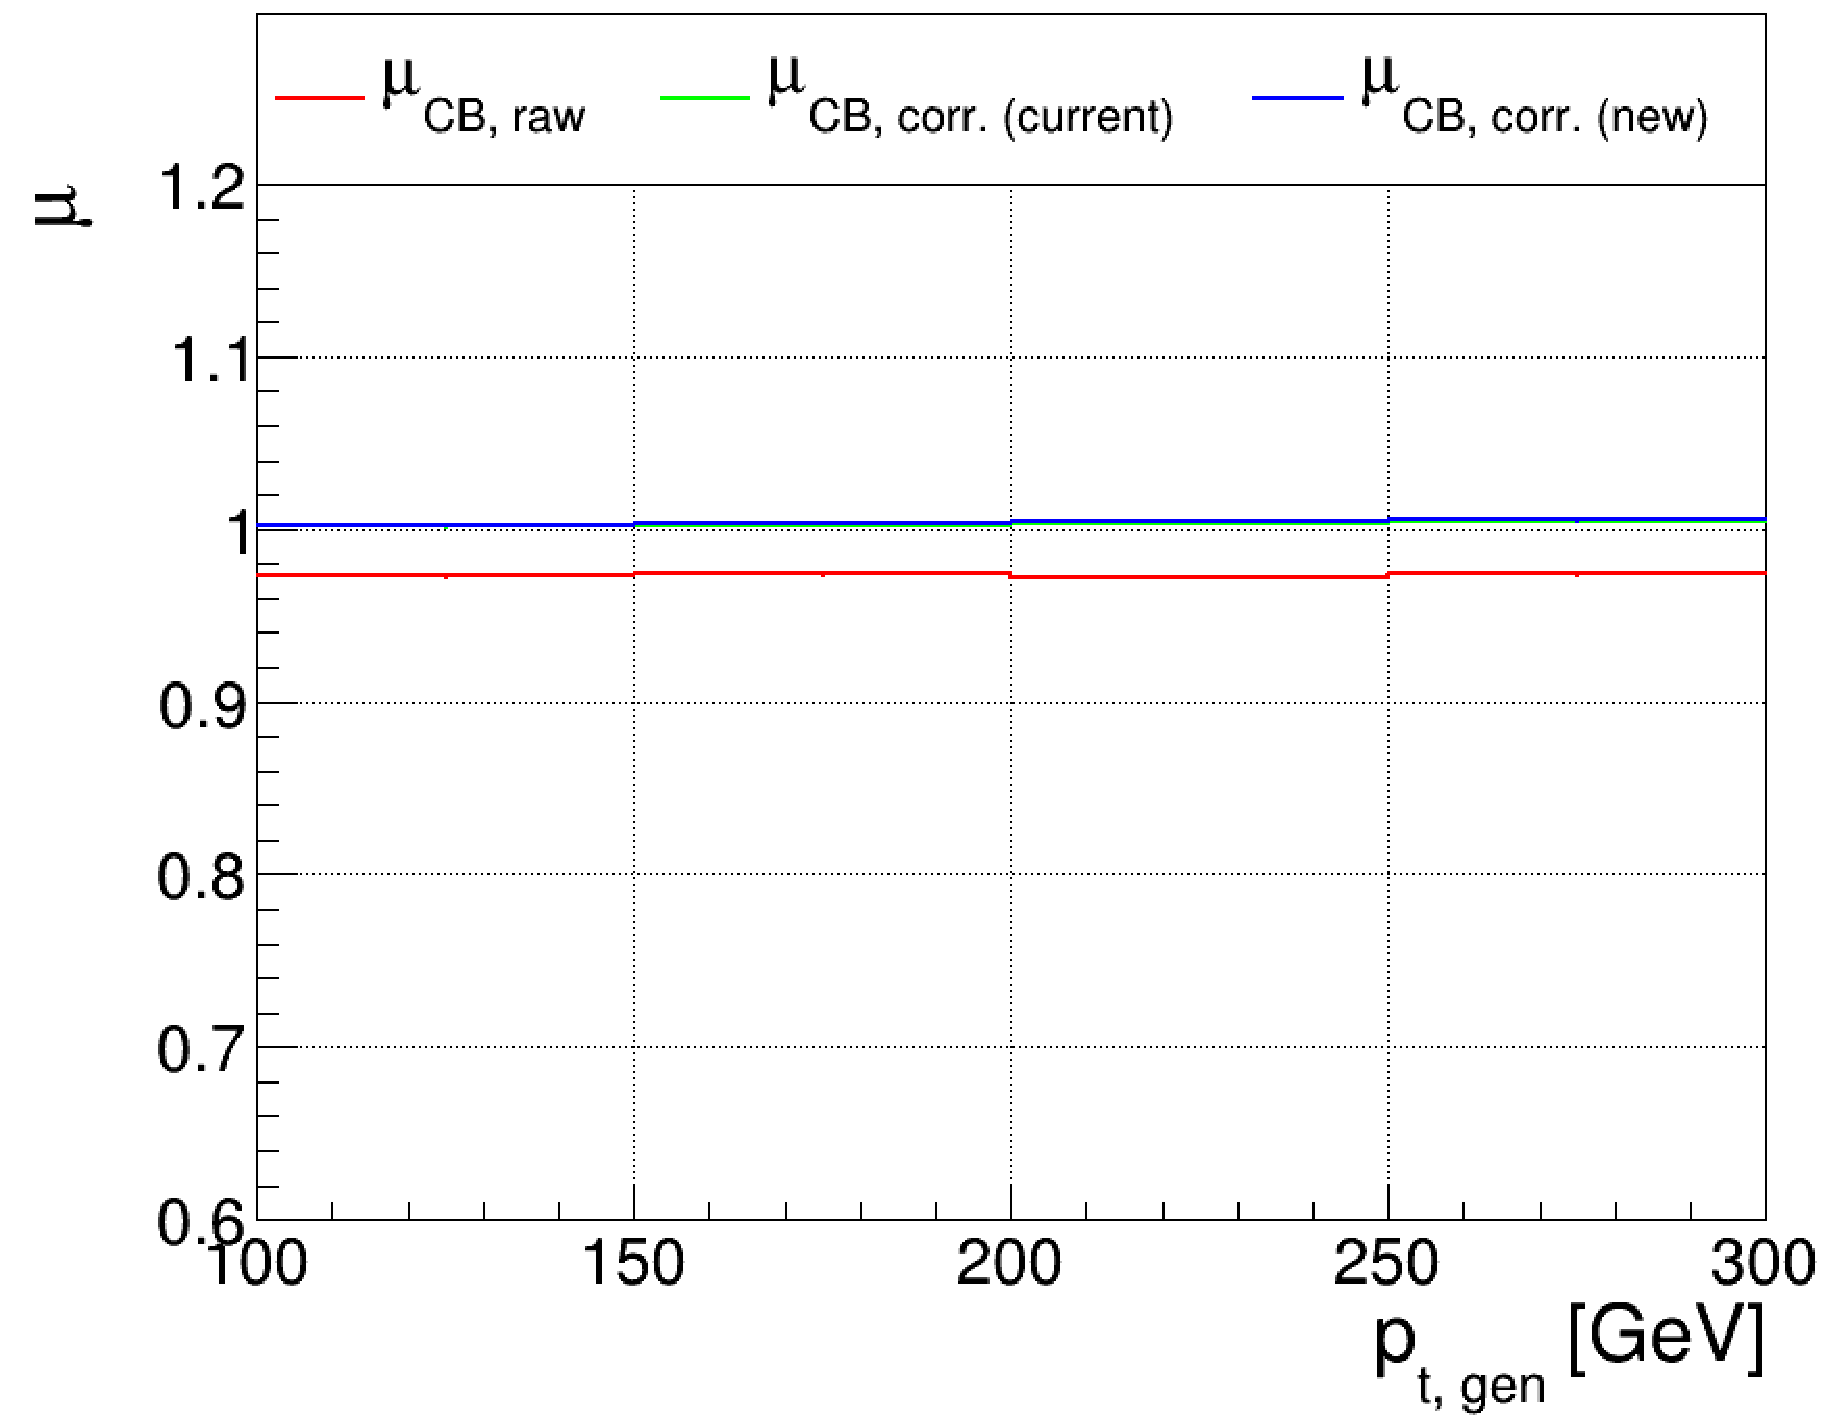
\includegraphics[width=0.495\textwidth]{./plots_pdf/ECAL_plots/plotsNoPU/EE/pdf/FULL/GENPT/EEFULL_GENPT_0100_0300_MuOverBins.pdf}
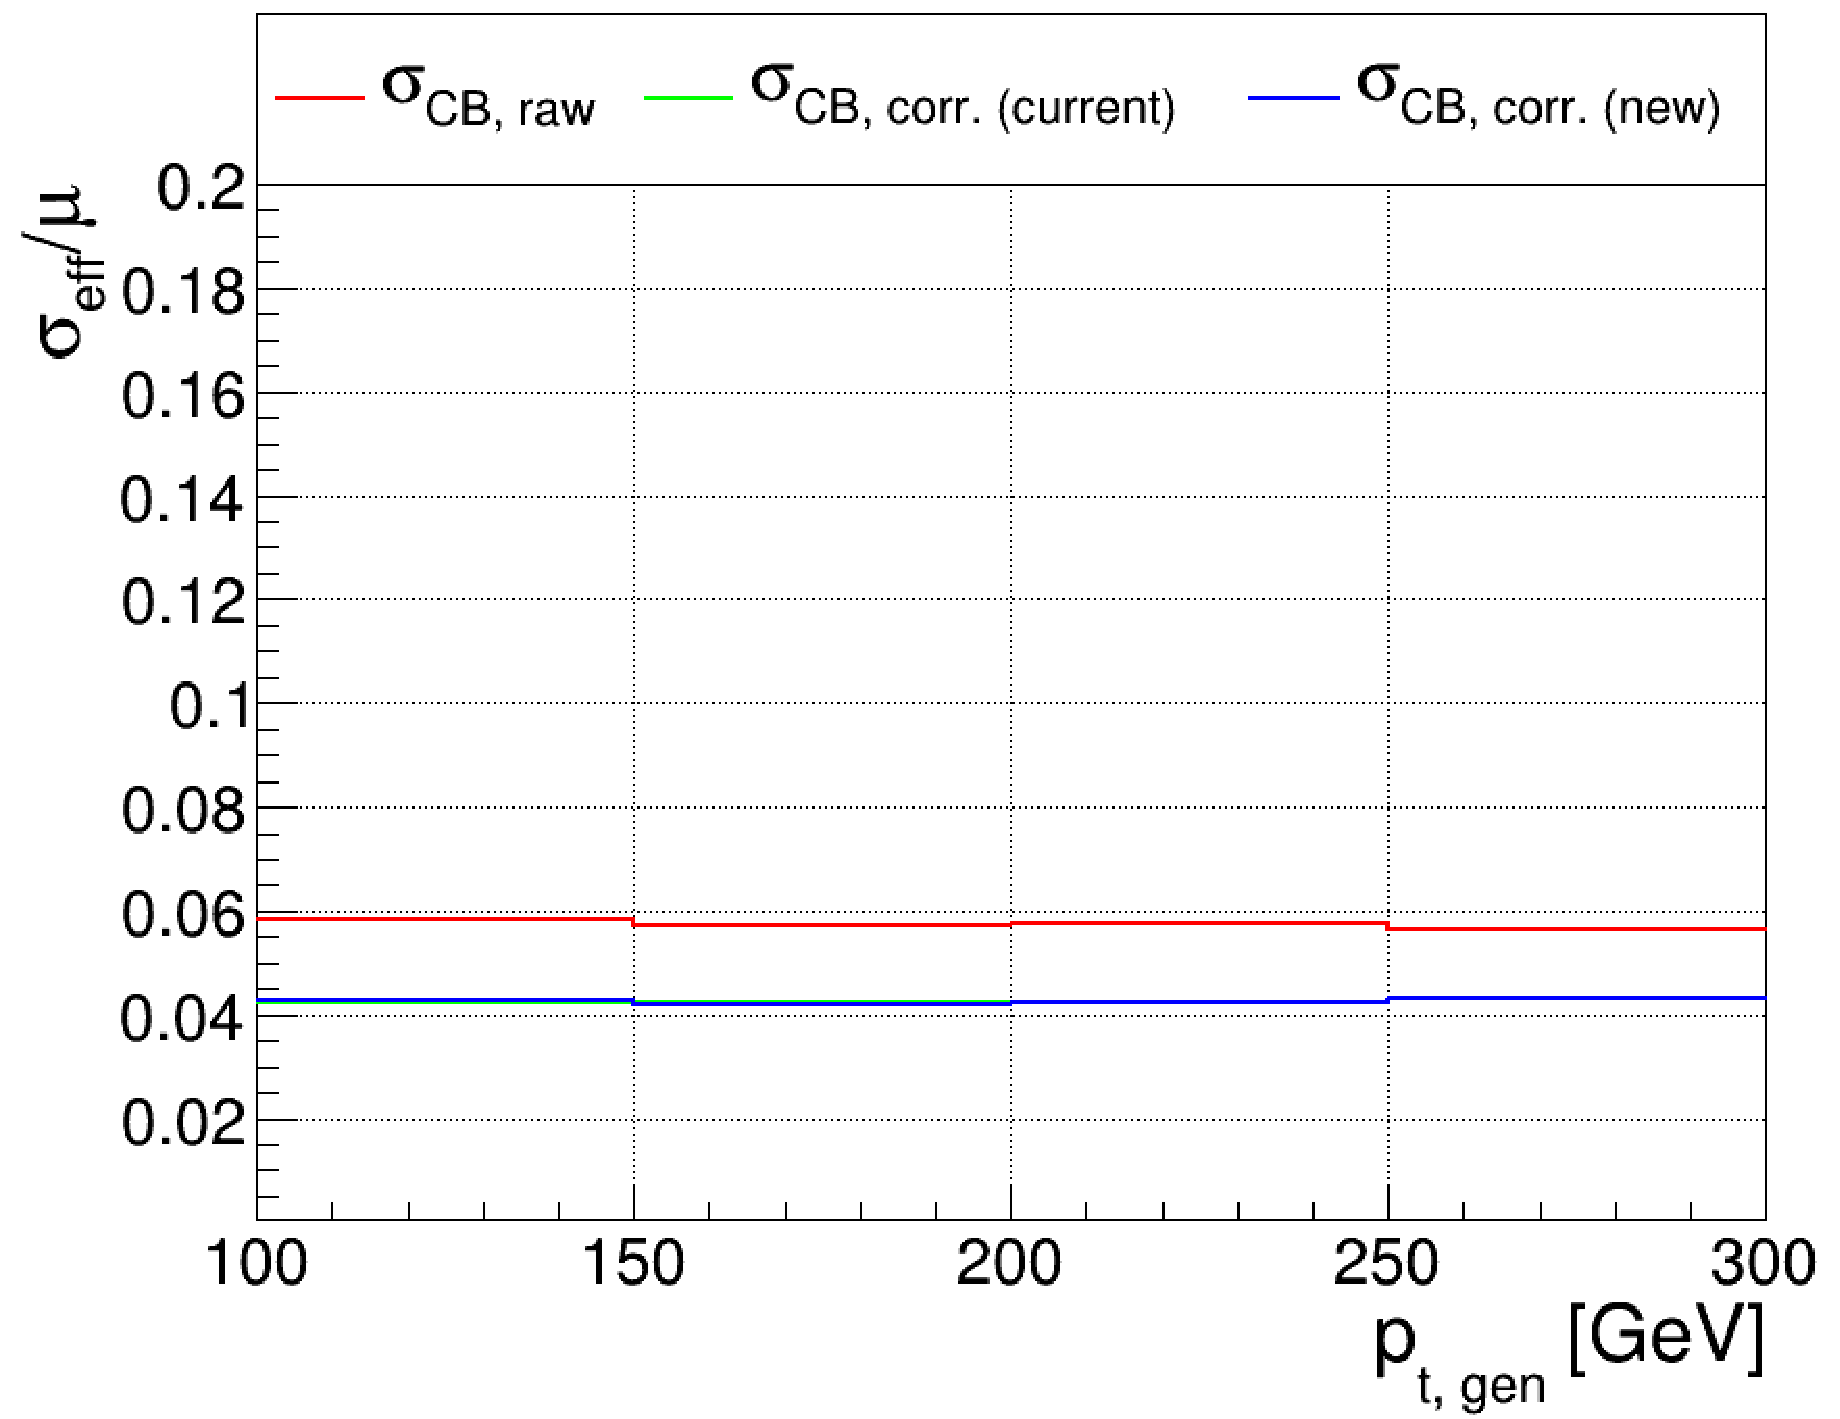
\includegraphics[width=0.495\textwidth]{./plots_pdf/ECAL_plots/plotsNoPU/EE/pdf/FULL/GENPT/EEFULL_GENPT_0100_0300_EffSigmaOverBins.pdf}


\caption [$\mu$ ($\sigma_\mathrm{eff}$) vs. \pt of PF ECAL cluster - EE full readout NoPU scenario]{Mean response (resolution) defined by raw PF ECAL clusters (red), the calibration derived earlier in Run~3 based on 126X (green), and the new correction from the 2024 simulation sample based on 133X (blue). (top) low \pt, (middle) mid \pt, (bottom) high \pt in EE region full readout NoPU scenario.}
\label{fig:NOPU_EEFULL_pt}
\end{figure}



\begin{figure}
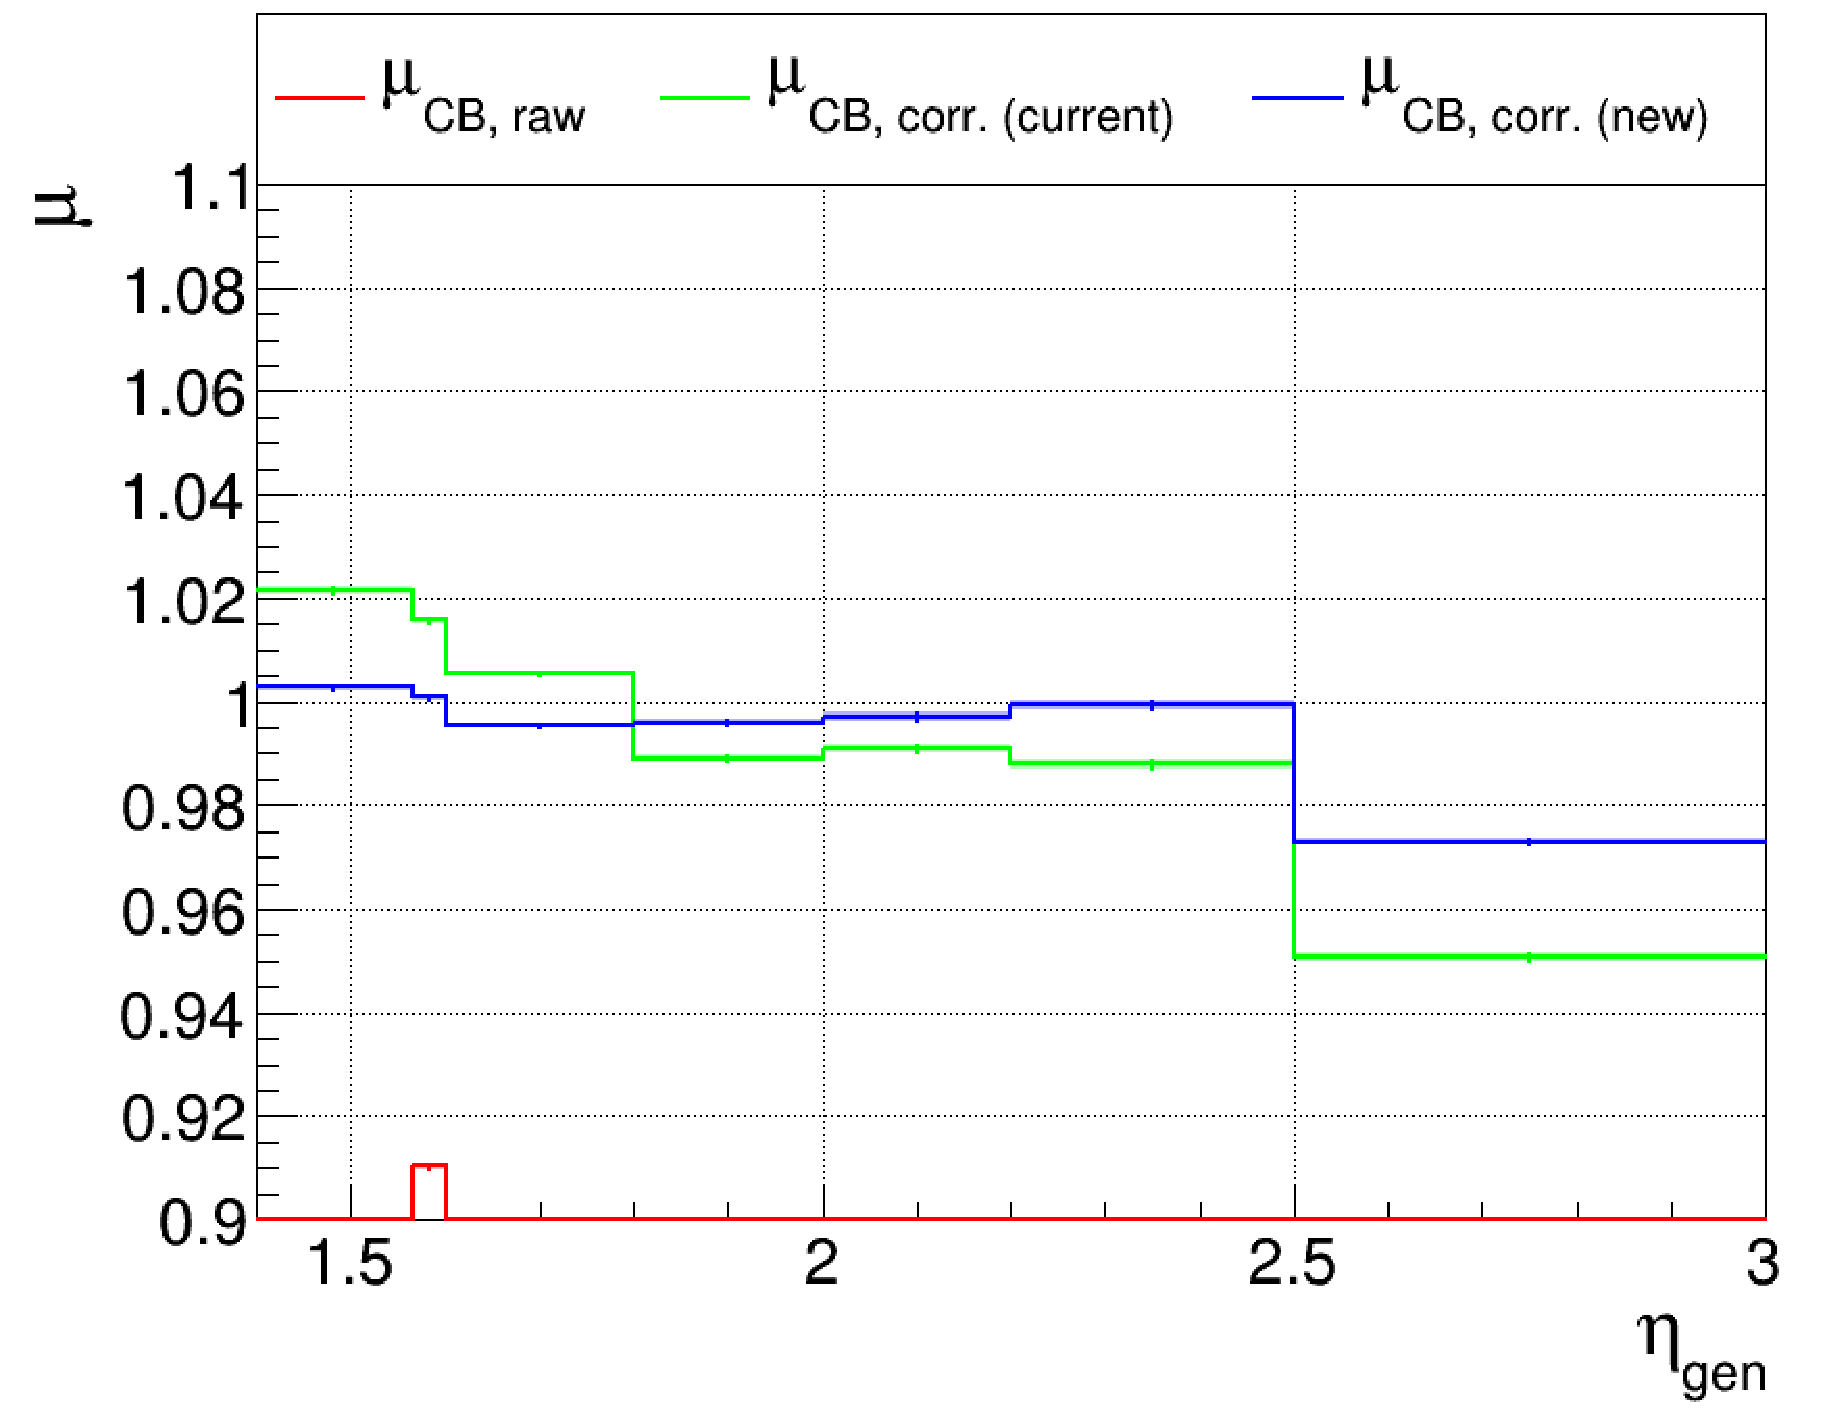
\includegraphics[width=0.495\textwidth]{./plots_pdf/ECAL_plots/plotsNoPU/EE/pdf/FULL/GENETA/EEFULL_GENETA_0005_0020_MuOverBins.pdf}
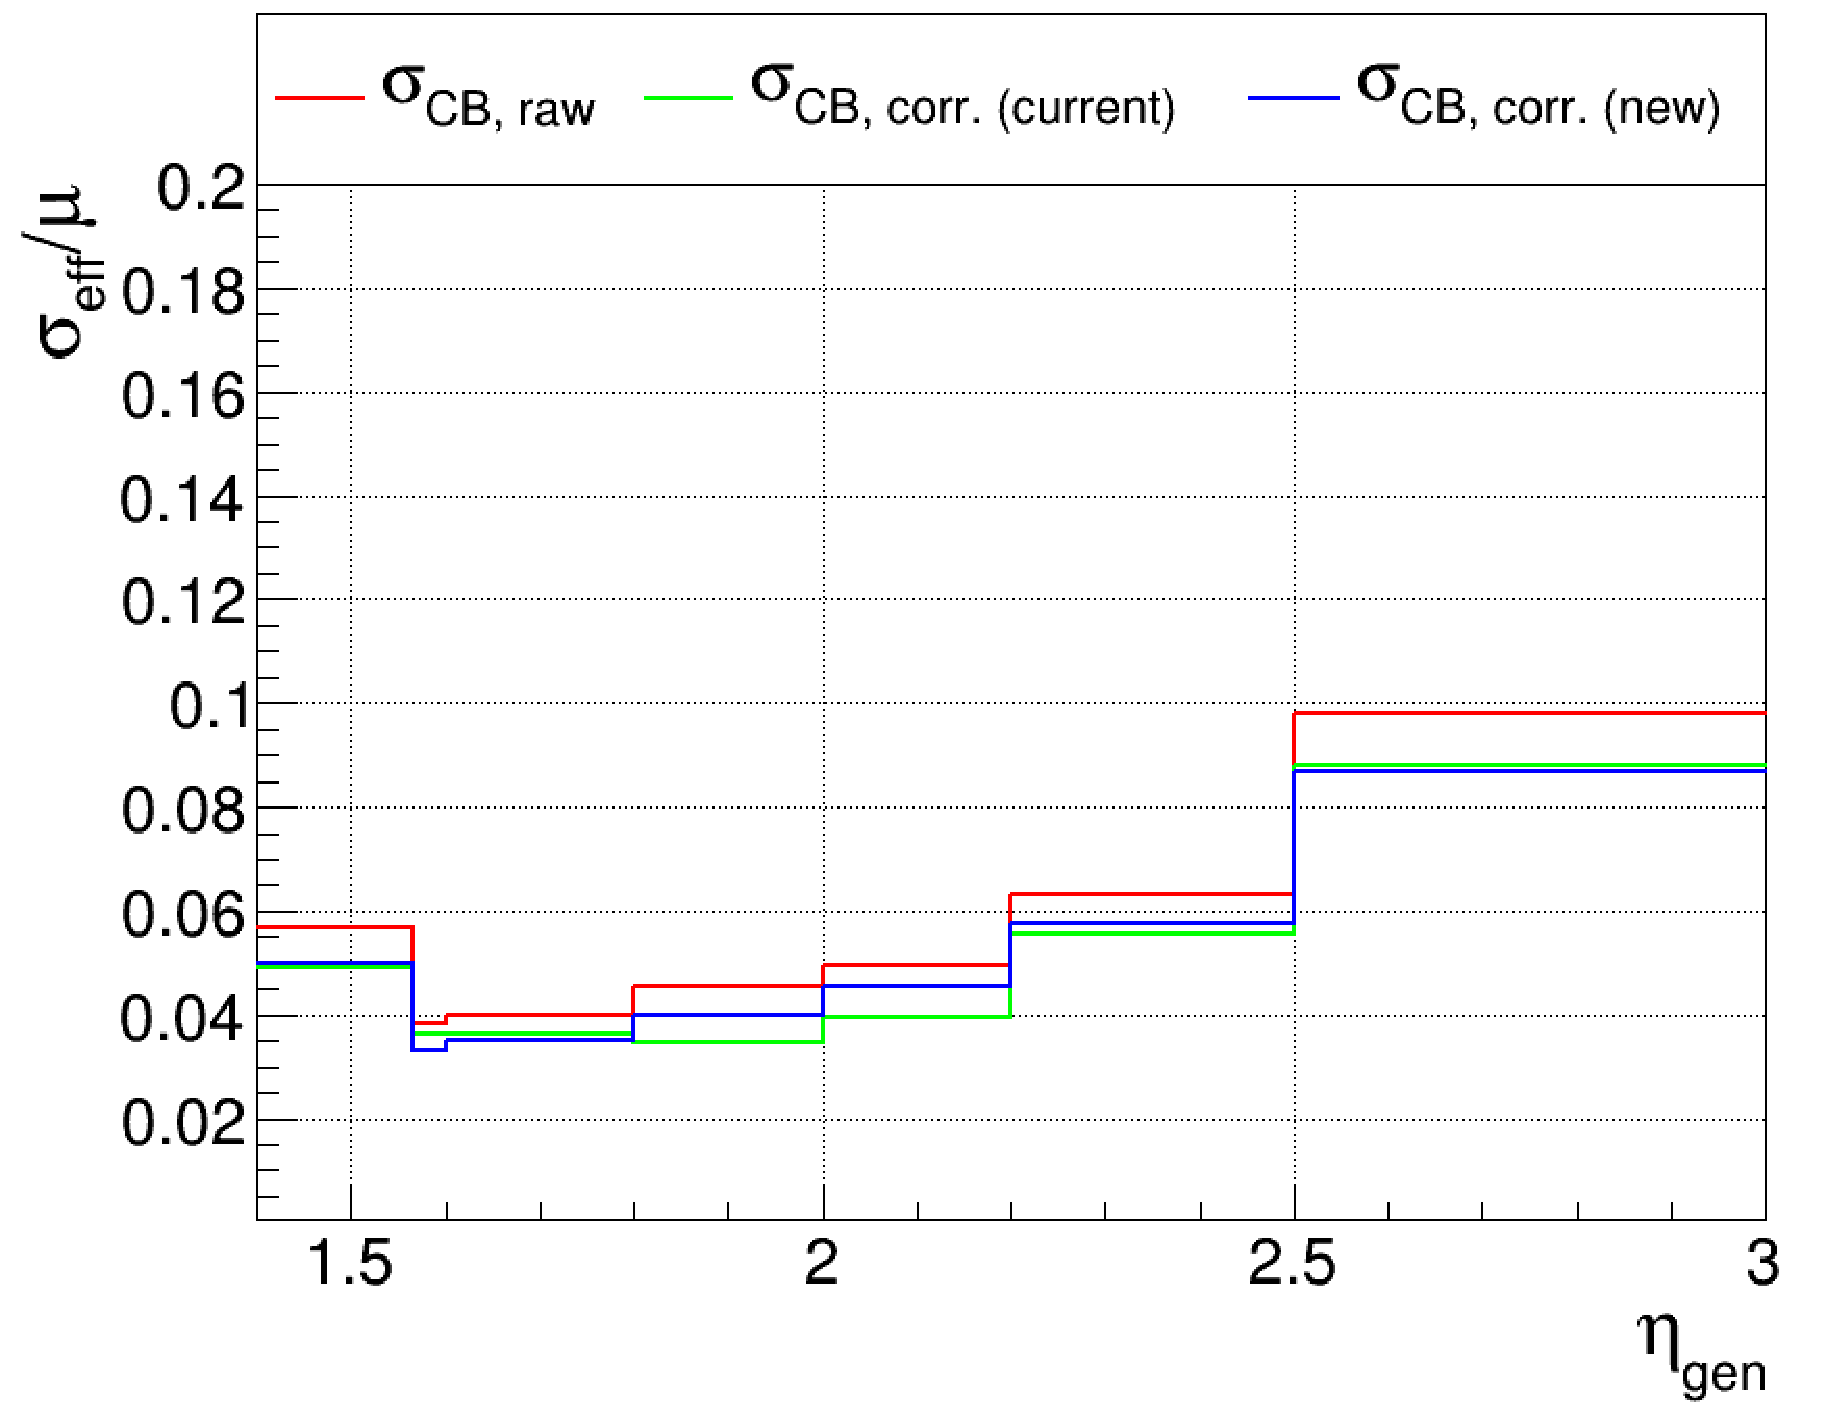
\includegraphics[width=0.495\textwidth]{./plots_pdf/ECAL_plots/plotsNoPU/EE/pdf/FULL/GENETA/EEFULL_GENETA_0005_0020_EffSigmaOverBins.pdf}
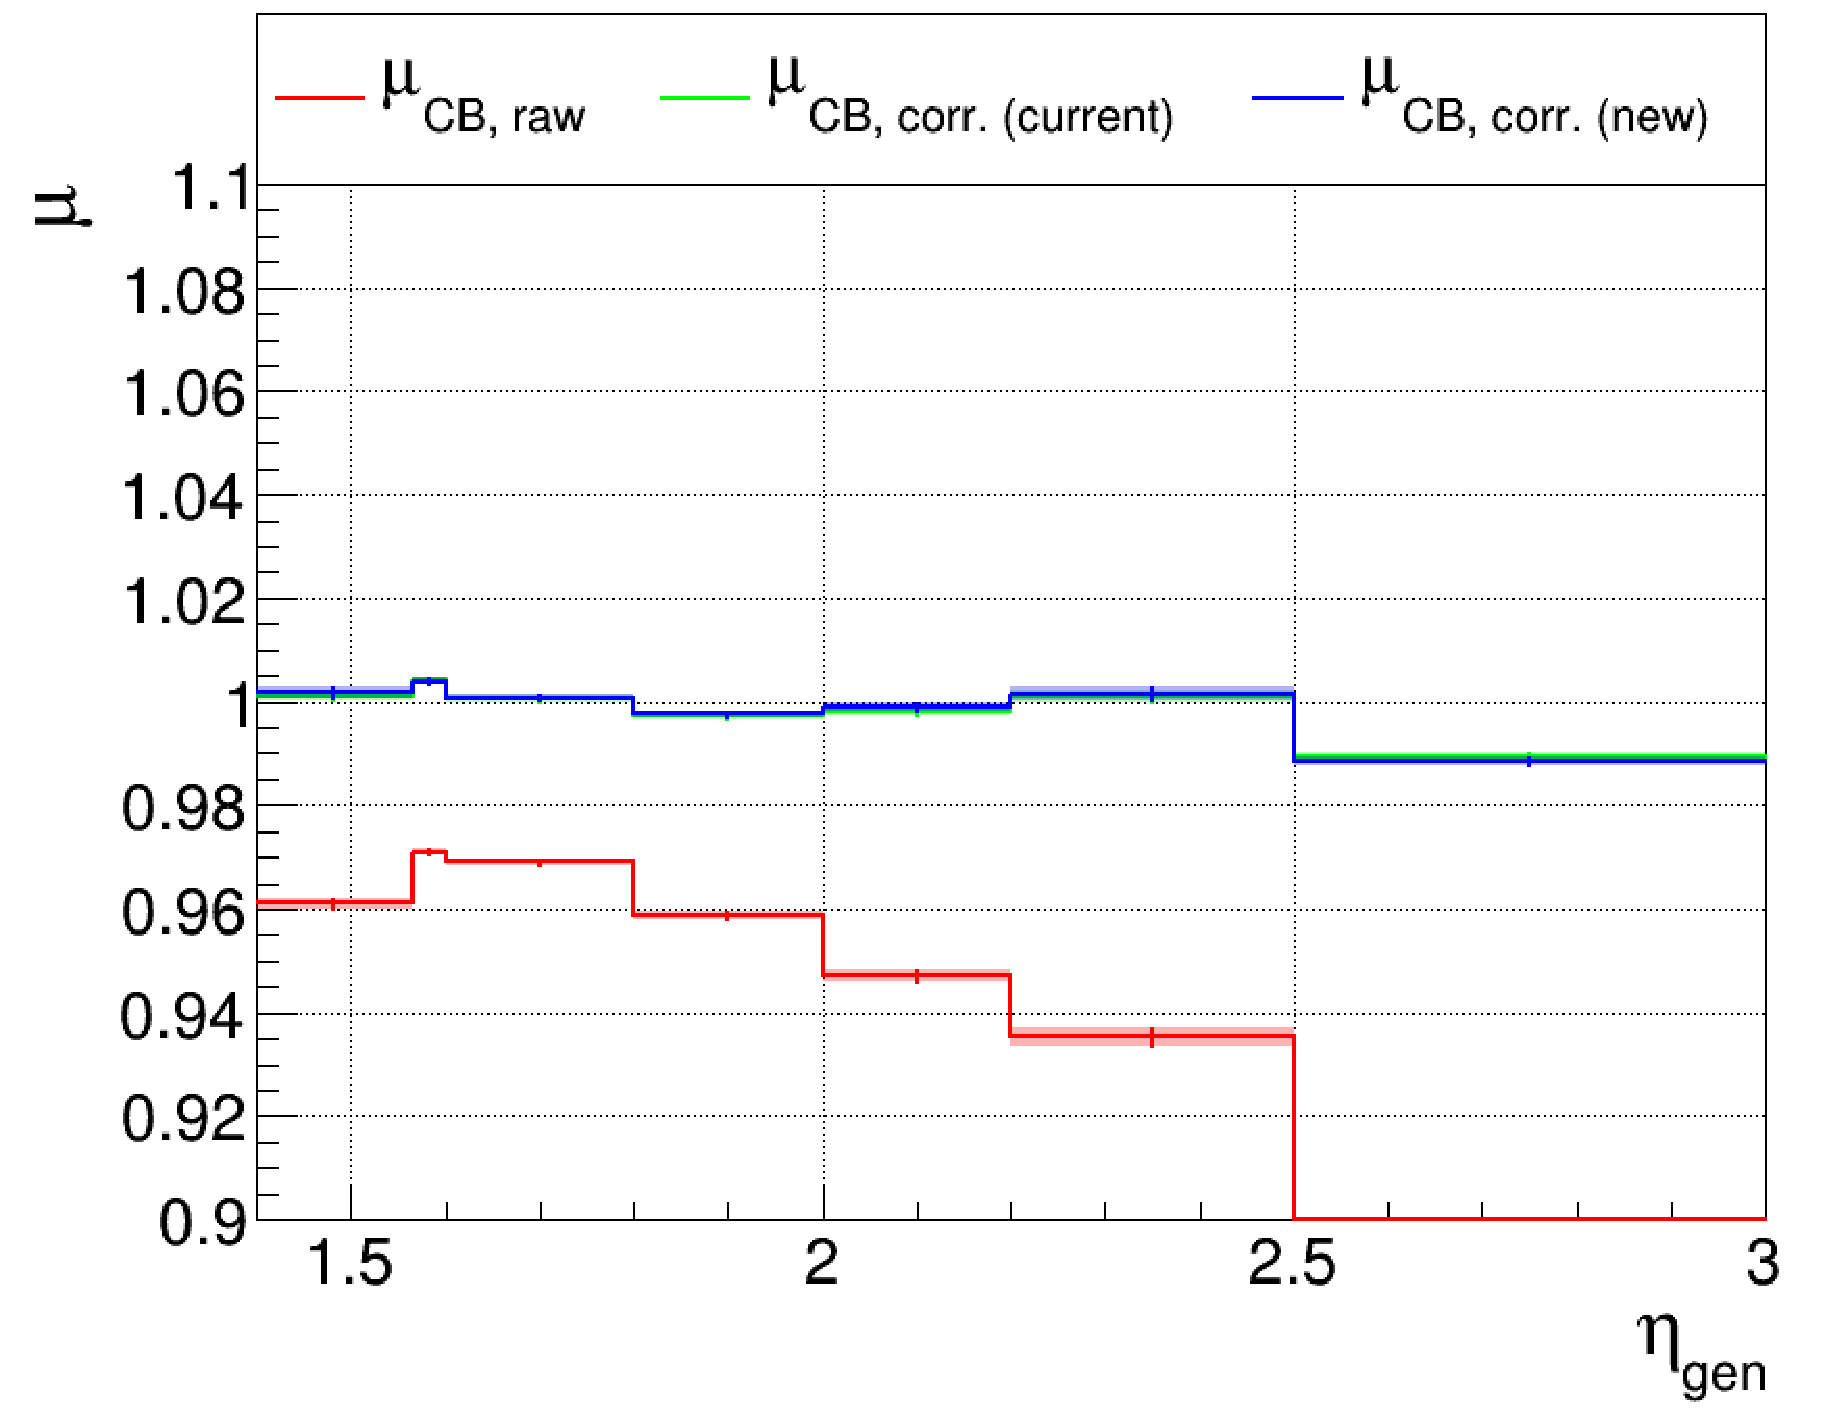
\includegraphics[width=0.495\textwidth]{./plots_pdf/ECAL_plots/plotsNoPU/EE/pdf/FULL/GENETA/EEFULL_GENETA_0020_0100_MuOverBins.pdf}
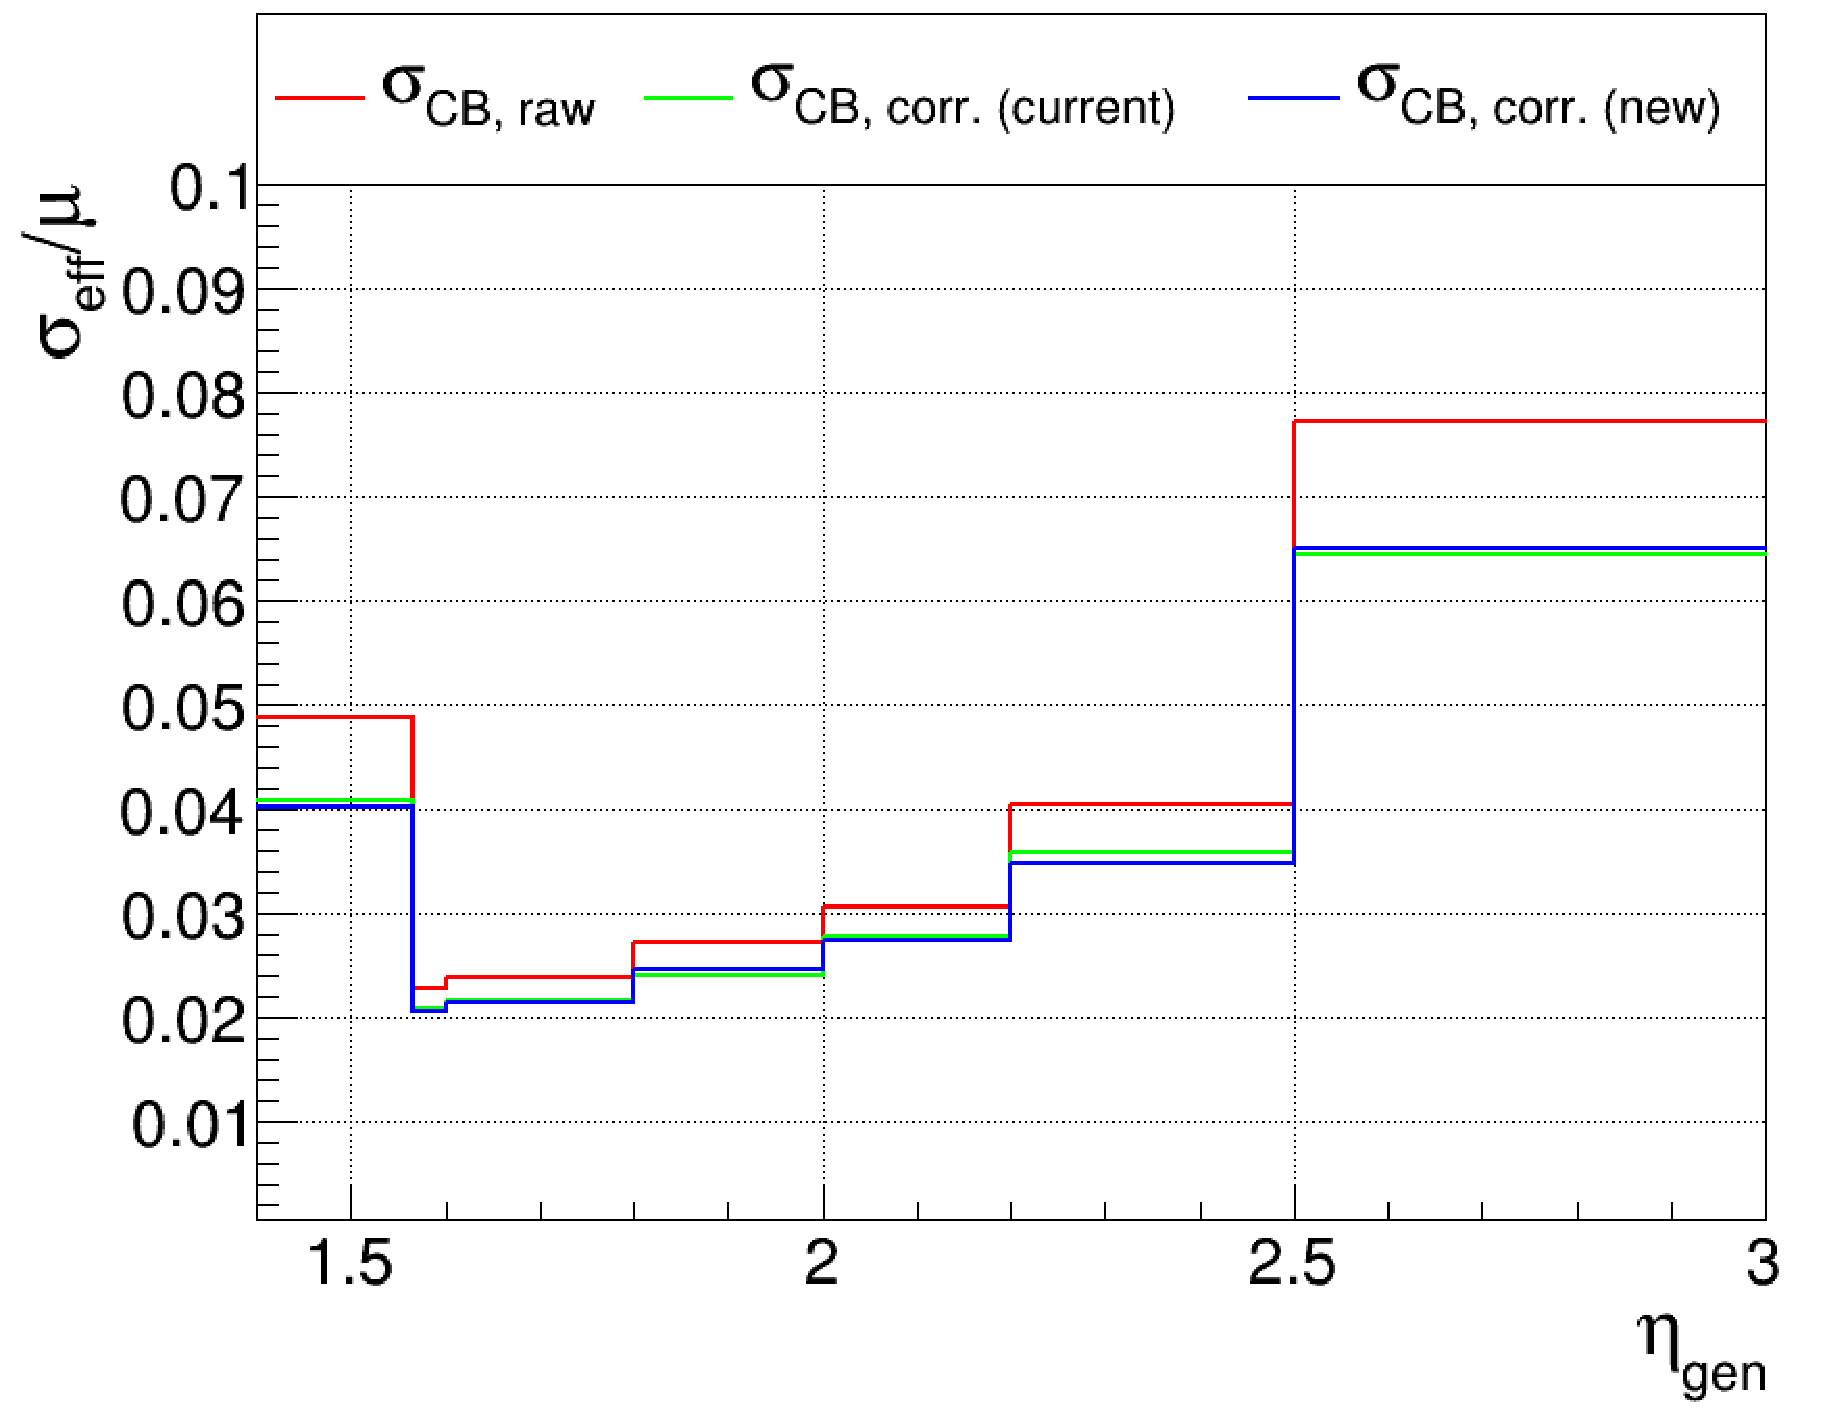
\includegraphics[width=0.495\textwidth]{./plots_pdf/ECAL_plots/plotsNoPU/EE/pdf/FULL/GENETA/EEFULL_GENETA_0020_0100_EffSigmaOverBins.pdf}
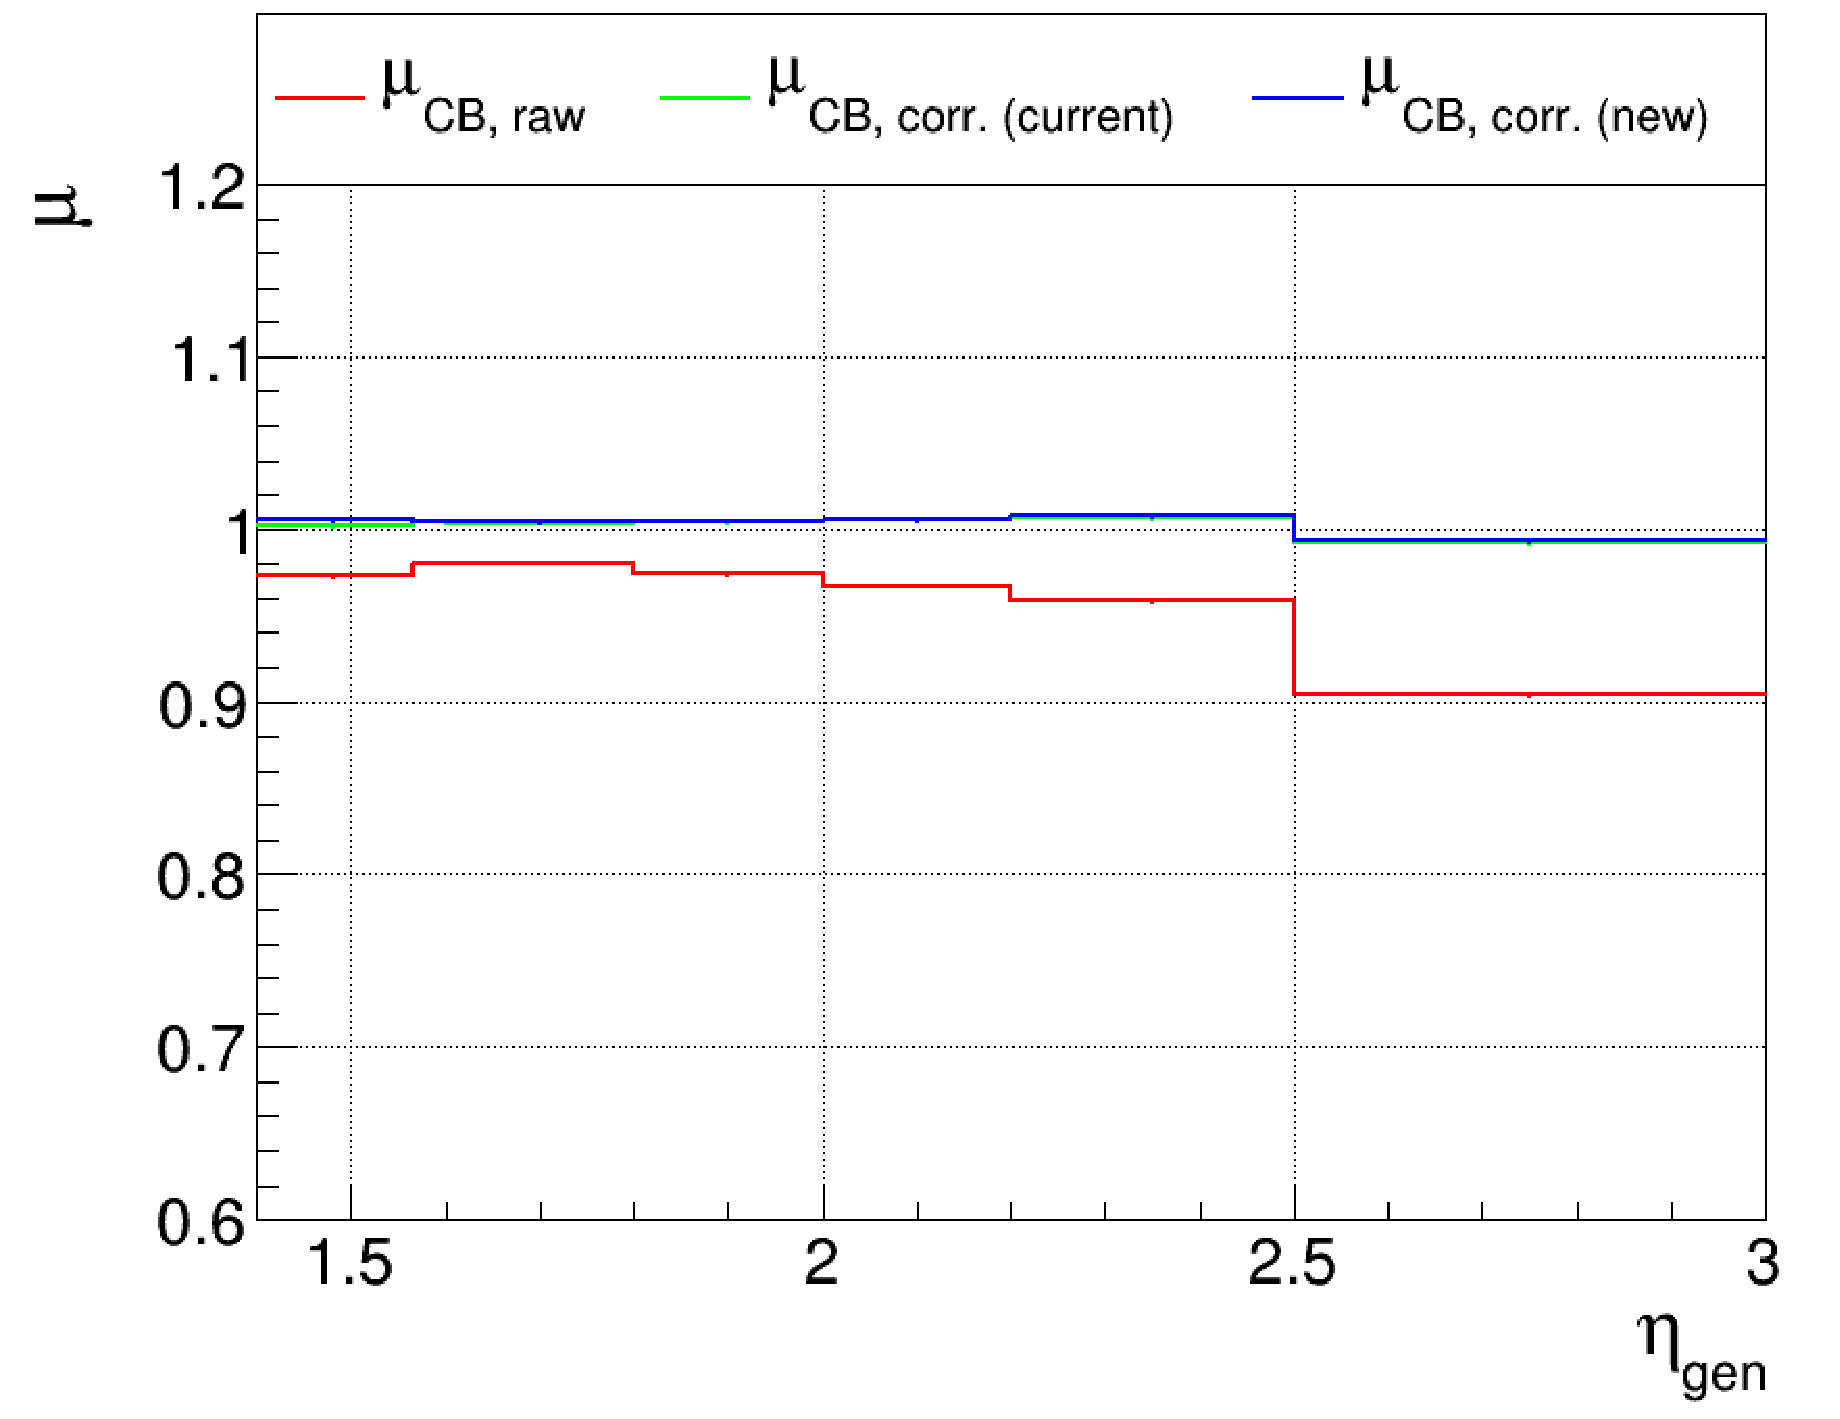
\includegraphics[width=0.495\textwidth]{./plots_pdf/ECAL_plots/plotsNoPU/EE/pdf/FULL/GENETA/EEFULL_GENETA_0100_0300_MuOverBins.pdf}
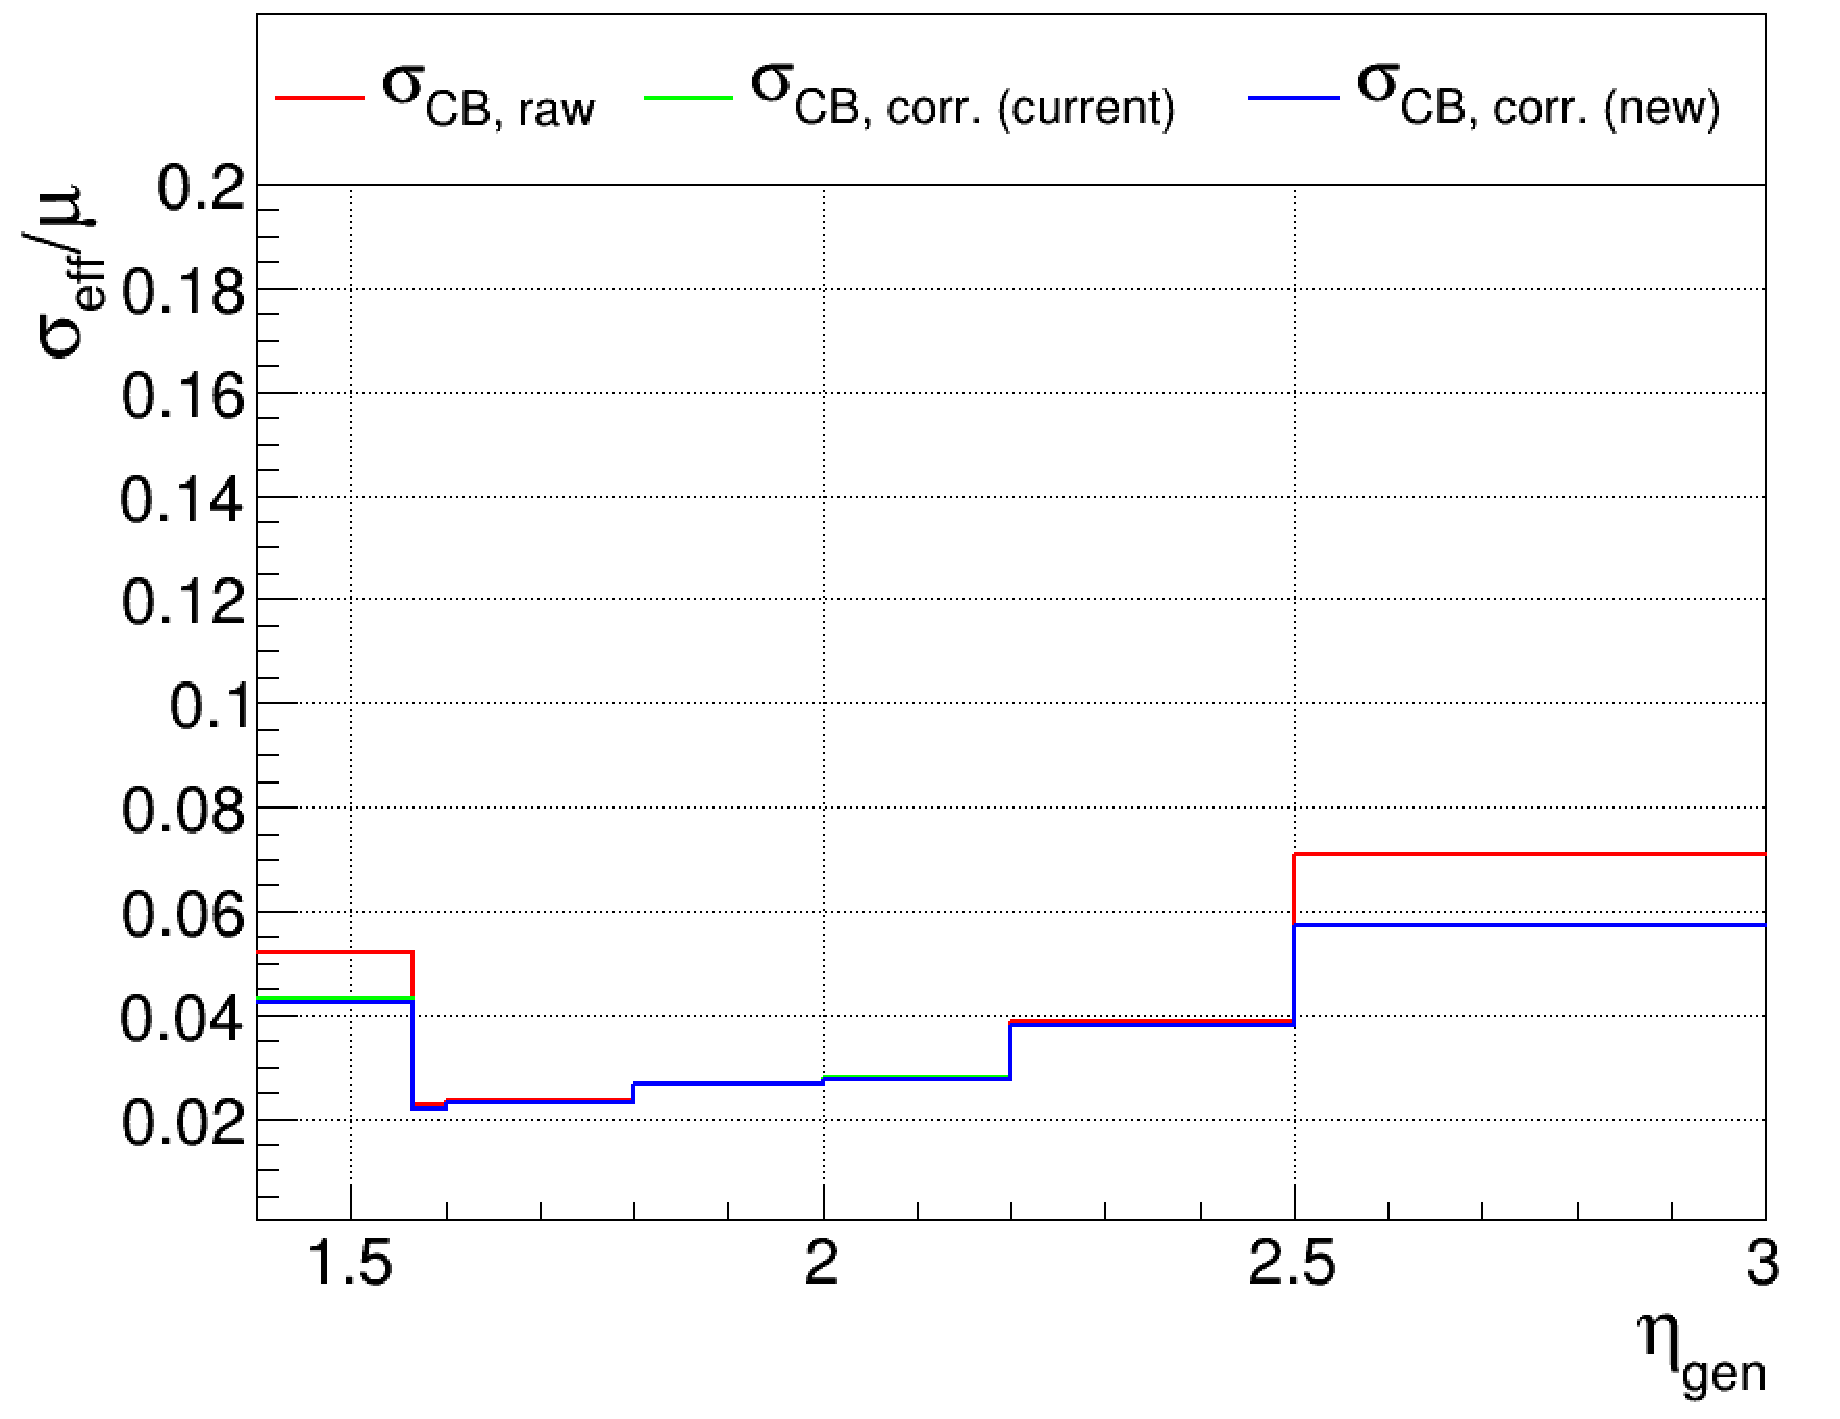
\includegraphics[width=0.495\textwidth]{./plots_pdf/ECAL_plots/plotsNoPU/EE/pdf/FULL/GENETA/EEFULL_GENETA_0100_0300_EffSigmaOverBins.pdf}

\caption [$\mu$ ($\sigma_\mathrm{eff}$) vs. $\eta$ of PF ECAL cluster - EE full readout NoPU scenario]{Mean response (resolution) defined by raw PF ECAL clusters (red), the calibration derived earlier in Run~3 based on 126X (green), and the new correction from the 2024 simulation sample based on 133X (blue). (top) low $\eta$, (middle) mid $\eta$, (bottom) high $\eta$ in EE region full readout NoPU scenario.}
\label{fig:NOPU_EEFULL_eta}
\end{figure}
